% -*-coding: utf-8 -*-



\defaultfont

\BiChapter{试验样机搭建与试验研究}{To Template Maintainers}
\BiSection{引言}{Simple Introduction about This Template}
\BiSection{试验样机硬件系统组成}{Subsubsection}
\BiSection{STM32底层电机驱动系统}{Subsubsection}
为了实现高层轨迹规划到底层电机的精准驱动，本研究设计并实现了基于 STM32 的多轴协同
控制系统。该系统向上对接 ROS 2 高级指令，向下通过精简的指令集控制伺服驱动器，构建
了高带宽、低延迟的底层控制基座。图\ref{pic61}为该系统的拓扑图


\begin{figure}[H] % htbp代表图片插入位置的设置
    \centering %图片居中
    %添加图片；[]中为可选参数，可以设置图片的宽高；{}中为图片的相对位置
    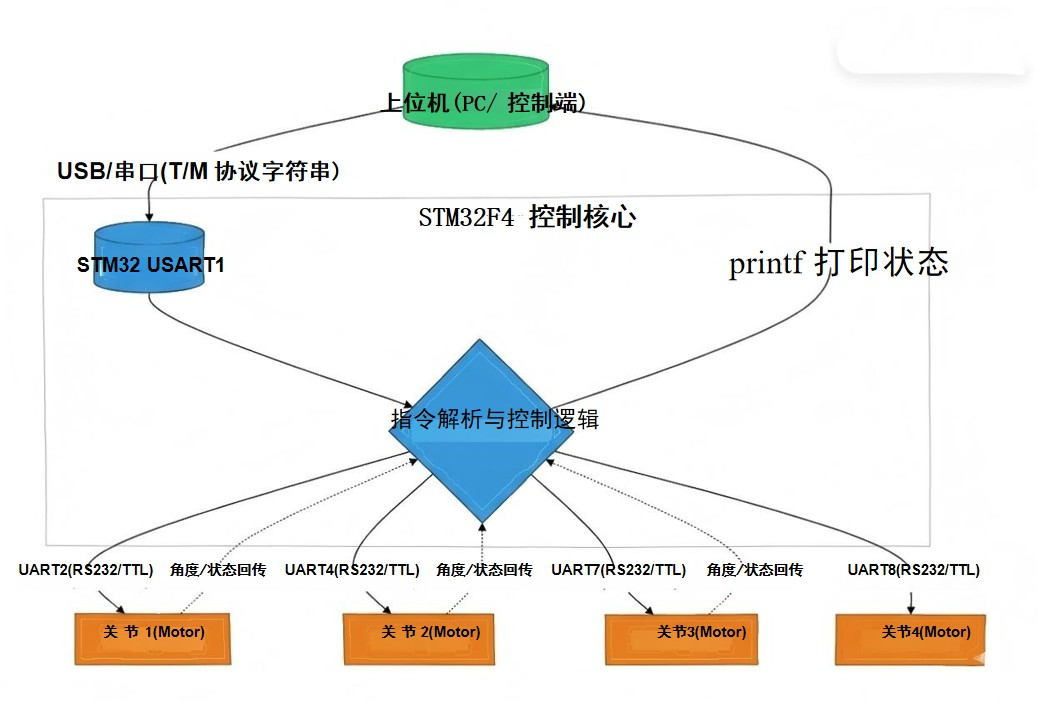
\includegraphics[width = 0.7\textwidth]{figures/stm.jpg}
    \caption{系统拓扑图} % 图片标题
    \label{pic61} % 图片标签
    \end{figure}


\BiSubsection{底层硬件架构与通信资源配置}{Hardware Architecture and Communication Configuration}
机械臂的底层控制系统以高性能的 STM32 微控制器为计算核心。其主频配置为 180\,MHz，通
过内部 PLL 倍频技术确保了控制算法在微秒级的快速迭代。

针对多关节机械臂的分布式控制需求，系统充分调动了 STM32 的多路通用同步收发传
输器（USART/UART）资源，构建了“中心化决策、分布式执行”的星型通信拓扑，具体配
置如下：

\begin{itemize}
    \item \textbf{上位机异构通信链路}：利用 USART1 与 ROS 2 上位机进行高速数据
    交互。为了有效缓解高频感知数据与控制指令并发产生的 CPU 负载压力，系统通过启
    用 \textbf{DMA（直接内存存取）循环缓冲机制} 配
    合 \textbf{串口空闲中断（IDLE Interrupt）}，实现了对非定长指令包的“无损”接收。
    该设计确保了即使在视觉算法高负载运行导致发包频率波动时，底层系统仍能维持控制链
    路的稳定性。
    \item \textbf{驱动器专用执行链路}：利用 USART2、UART4、UART7 与 UART8 建立四
    路物理隔离的执行通道，分别驱动各伺服关节。采用硬件抽象层（HAL）封装的数组化
    管理模式（\texttt{joint\_uart[4]}），不仅显著降低了多路中断调度冲突的概率，也
    为未来机械臂自由度的平滑扩展提供了软件接口保障。
\end{itemize}

\BiSubsection{多级通信协议与解析机制设计}{Multi-level Communication Protocol and Parsing}
为了确保异构系统间（Linux 实时环境与嵌入式裸机环境）控制流的语义一致性，系统设计了
双层通信协议架构。

（1）应用层文本协议解析 (ROS 2 $\leftrightarrow$ STM32)

在 \texttt{HAL\_UART\_RxCpltCallback} 中断服务程序中，系统集成了具备容错能力的
指令解析器。系统通过识别起始符与结束符，对接收到的文本帧进行实时反序列化：
\begin{enumerate}
    \item \textbf{绝对角度控制（T 协议）}：格式为
    \texttt{T,Angle1,N,Angle2,N,Angle3}。系统解析出绝对位姿后，会将其映射至驱动器
    的位置模式（Position Profile Mode），用于执行全局轨迹规划指令。
    \item \textbf{增量步进控制（M 协议）}：格式为 
    \texttt{M,Angle1,N,Angle2,N,Angle3}。该协议优先满足手动调试与细微示教需求，
    通过计算相对当前位置的角度偏移量，实现高精度的微量位移。
\end{enumerate}
系统内置了解析校验状态机，能自动过滤因物理层电气噪声产生的非法字符，防止错误的电机
动作造成机械损坏。

（2）底层总线协议与鲁棒性保障 (STM32 $\leftrightarrow$ 伺服电机)

单片机与驱动器间采用紧凑型十六进制报文通信。为应对复杂工业电磁环境下的数据篡改
风险，系统在物理层之上构建了基于 CRC-8 的数据一致性检查。其核心校验多项式设定
为 $0xD5$，位运算递推模型如式 (\ref{eq:crc8}) 所示：

\begin{equation}
\label{eq:crc8}
u8CRC_{n+1} =
\begin{cases}
(u8CRC_n \gg 1) \oplus 0xD5 & \text{if } (u8CRC_n \wedge 0x01) \neq 0 \\
u8CRC_n \gg 1 & \text{otherwise}
\end{cases}
\end{equation}

该机制不仅验证了指令字，亦对关键参数位（如期望角度、限制电流）进行全域校验，确保
了控制指令执行的原子性。

\BiSubsection{关节运动控制策略实现}{Joint Motion Control Strategy Implementation}
（1）初始化与自校准逻辑 (Homing)

系统初始化流程遵循“先使能、后寻标”的逻辑。通过 \texttt{joint\_init()} 配置驱动器内
部参数（如加速斜率、过载保护阈值）。由于绳驱系统存在断电位姿丢失的问题，系统执
行 \texttt{joint\_homing()} 函数，利用硬件限位或编码器索引脉冲触发驱动器的归零

模式（Homing Mode）。针对不同轴向的机械行程差异，通过配置对象字典 \texttt{0x6098} 
分配特定的回零搜索路径，从而建立统一的笛卡尔坐标系基准。

（2）精细化动力输出与转换

在执行指令时，系统通过 \texttt{joint\_move()} 等接口实现从逻辑角度到物理脉冲的转化：
\begin{itemize}
    \item \textbf{数据对齐}：针对 16 位控制字，系统采用
     \textbf{小端模式（Little-endian）} 自动完成数据的拆分与重组，确保字节序在总
     线传输中的一致性。
    \item \textbf{方向自适应映射}：根据设定角度的代数符号，自动反转报文的方向位
    掩码。此举通过软件层屏蔽了电机安装方向不一致带来的控制复杂度，简化了上层运动
    学模型的极性判断。
\end{itemize}

（3）双向反馈闭环与同步监控

系统不仅是指令的发布方，亦是状态的监控者。系统以 30\,ms 为固定周期触发轮询中断，
周期性主动索取驱动器的状态字。利用位移运算重构实际角度反馈值，如式
 (\ref{eq:angle_calc}) 所示：

\begin{equation}
\label{eq:angle_calc}
\text{Real\_Angle} = (\text{RxPacket}[8] \ll 8) \mid \text{RxPacket}[7]
\end{equation}

该实时数据流被反向传输至 ROS 2 节点，用
于维持物理样机的状态同步，并为基于视觉反馈的抓取误差补偿提
供高频位置参考。

\BiSection{基于 ROS 2 的控制系统软件设计}{Software Design of Control System Based on ROS 2}

本研究基于 ROS 2分布式架构设计了机械臂的控制系统软件平台。系统利用 ROS 2 的通讯机制实现了感知、决策与执行的高度解耦，构建了从视觉交互到物理执行的完整自动化作业链路。

\BiSubsection{系统总体逻辑架构}{Overall System Logic Architecture}

控制系统整体由一系列独立的计算节点组成，通过话题、服务及动作进行交互。如图 \ref{pic62} 所示（此处引用您的流程图），系统逻辑可分为四个功能层：
\begin{enumerate}
    \item \textbf{感知层}：负责实时图像采集、目标物体框选交互及坐标解算。
    \item \textbf{调度层}：维护机械臂抓取作业的有限状态机，指挥任务序列。
    \item \textbf{规划层}：包含 G 代码解释器、直线/圆弧插补服务及逆运动学（IK）服务。
    \item \textbf{执行层}：负责串口协议封装及与下位机 STM32 的双向握手。
\end{enumerate}
\begin{figure}[H] % htbp代表图片插入位置的设置
    \centering %图片居中
    %添加图片；[]中为可选参数，可以设置图片的宽高；{}中为图片的相对位置
    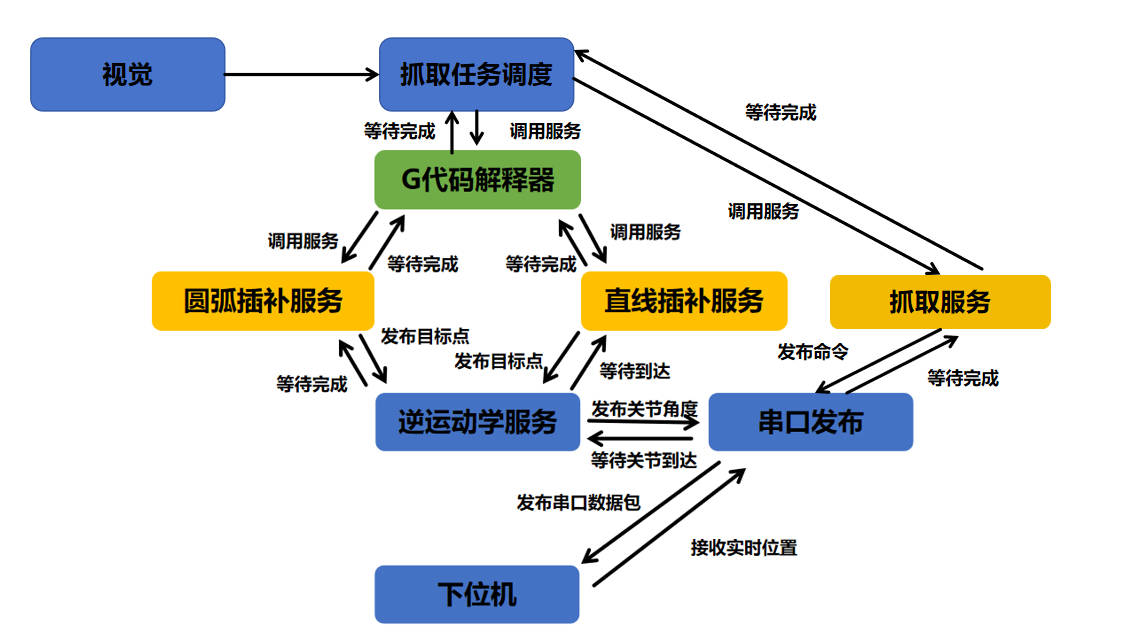
\includegraphics[width = \textwidth]{figures/ros2.jpg}
    \caption{系统拓扑图} % 图片标题
    \label{pic62} % 图片标签
    \end{figure}

\BiSubsection{视觉监控与目标交互定位模块}{Vision Monitoring and Target Interactive Positioning}

为实现非结构化环境下的自主抓取，本研究开发了基于 OpenCV 与交互式界面的视觉定位节点。

（1）实时图像监视与 ROI 框选交互

视觉节点通过高帧率相机获取作业现场。系统通过鼠标回调函数实现用户交互：操作者在监控界面通过鼠标拖拽划定感兴趣区域（ROI）。系统实时提取框选区域的质心像素坐标 $(u_c, v_c)$，并将其作为目标输入的初始值。

（2）空间坐标解算模型

基于单目视觉标定模型，结合预先完成的手眼标定，将图像坐标映射至机械臂基座坐标系 $O_{base}$。设像素坐标为 $P_{uv}$，则其在机械臂基座坐标系下的位姿 $P_{base}$ 可通过式 (\ref{eq:eye_to_base}) 描述：
\begin{equation}
\label{eq:eye_to_base}
P_{base} = T_{eye}^{base} \cdot (K^{-1} \cdot s \cdot P_{uv})
\end{equation}
其中，$K$ 为相机内参矩阵，$T_{eye}^{base}$ 为手眼转换矩阵，$s$ 为深度比例因子。

\BiSubsection{抓取任务调度状态机设计}{Design of Grasping Task Dispatching State Machine}

调度节点 \texttt{task\_manager} 是系统的核心，负责管理抓取作业的全生命周期。为了保证作业的稳健性，设计了如下状态机：

\begin{itemize}
    \item \textbf{待机状态}：系统完成自检，循环监听视觉节点发布的坐标信息。
    \item \textbf{靠近状态}：获取目标坐标后，调度节点计算预抓取点（目标上方 5\,cm），并调用运动规划服务控制机械臂快速靠近。
    \item \textbf{执行抓取}：机械臂到达预定点后，指令执行下降并触发执行器闭合，同时监测反馈以确认抓取成功。
    \item \textbf{搬运状态}：规划至预设放置点的平滑轨迹，避开可能存在的机械限位。
    \item \textbf{复位状态}：释放目标物，机械臂沿安全高度返回零点，等待下一轮框选指令。
\end{itemize}

\BiSubsection{基于 G 代码的运动规划模块实现}{Implementation of Motion Planning Based on G-code}

本模块负责将调度节点下发的位姿指令转化为连续的关节运动指令。

（1）G 代码解释与轨迹插补

系统支持标准 G 代码指令集。解释器将 $G01$（直线）或 $G02/G03$（圆弧）指令解析后，由插补服务实时生成路径点。插补频率可修改，确保了末端执行器轨迹的平滑性。

（2）逆运动学服务与反馈同步

插补点作为客户端请求发送至 \texttt{ik\_service} 节点。该节点根据三自由度机械臂的运动学解析模型，求解对应的关节角度组 $\{\theta_1, \theta_2, \theta_3\}$。为防止指令堆积导致控制失稳，插补服务与下位机之间通过“等待到达”信号实现严格的时间同步，如图 \ref{pic62} 中的双向箭头所示。

\BiSubsection{串口通信发布与闭环状态监测}{Serial Communication and Closed-loop Monitoring}

串口发布节点作为上位机与 STM32 的通讯门户。其核心逻辑包括：
\begin{itemize}
    \item \textbf{协议封装}：将规划角度编码为特定帧格式，包含校验位以防止数据误读。
    \item \textbf{实时反馈映射}：接收 STM32 反馈的实时脉冲数据，反解为实际角度，并通过 节点发布。这一过程实现了物理样机到控制系统的同步。同时，便于实验者直观监视运动状态。
\end{itemize}


\BiSection{机械臂基本运动性能试验}{Subsubsection}
\BiSubsection{实验环境与平台}{Experimental Environment and Platform}
实验于机电工程学院实验室开展。实验平台主要由水下绳驱机械臂原型、控制系统终端、高精度摄像机组成。实验环境光照稳定，背景纹理清晰，符合视觉算法的测试要求。

\BiSubsection{实验内容与流程}{Experimental Content and Process}
为全面验证机械臂的运动性能及控制算法的有效性，本研究开展了如下实验流程：
\begin{enumerate}
    \item \textbf{基础运动测试}：通过控制台指令完成机械臂的系统复位，验证各关节在工作空间内的独立运动性能。
    \item \textbf{运动学与轨迹规划验证}：利用逆运动学解算算法，给定末端目标位姿，测试机械臂在笛卡尔空间下的轨迹规划能力（如直线与圆弧插补）。
    \item \textbf{视觉引导下的闭环抓取实验}：集成 OpenCV 与 ROS2 环境下的视觉定位节点，利用 Aruco 码对目标物进行识别与定位，驱动机械臂完成自动抓取任务。
\end{enumerate}

\begin{figure}[H]
    \centering
    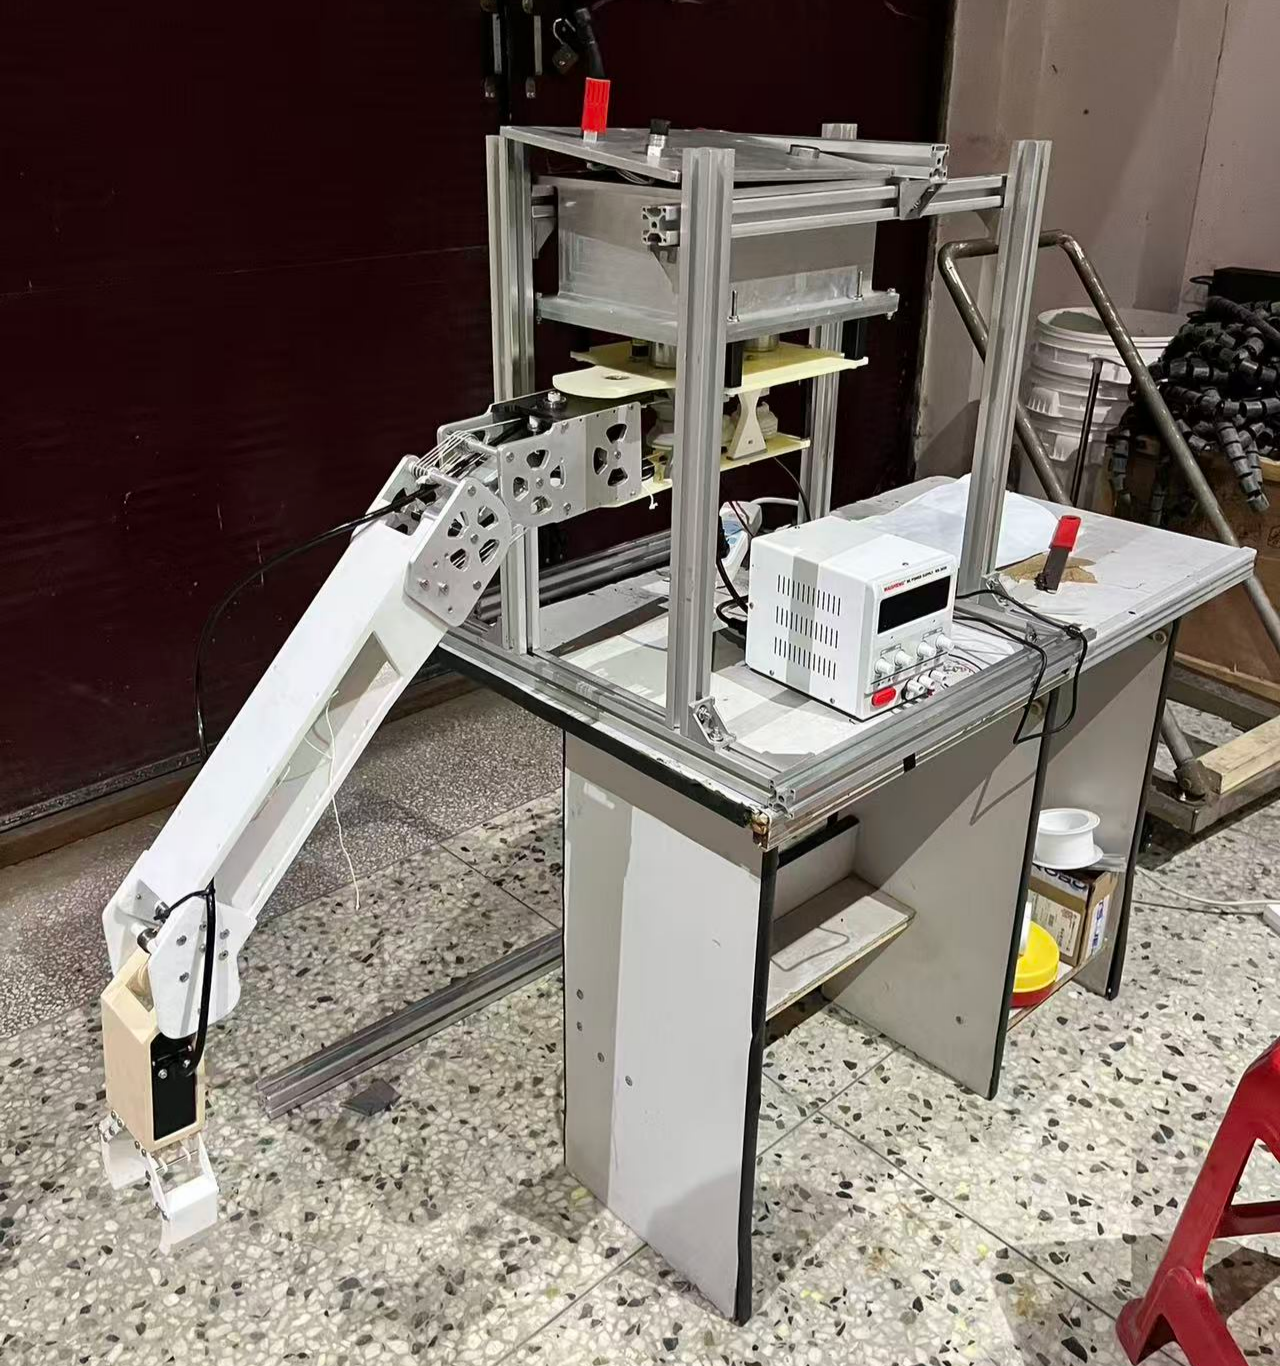
\includegraphics[width=0.7\textwidth]{figures/轴测图.jpg}
    \caption{机械臂运动学验证与轨迹规划实验现场}
    \label{fig:motion_test}
\end{figure}

\BiSubsection{实验结果与误差分析}{Experimental Results and Error Analysis}
实验结果表明，该系统具有较好的鲁棒性与可靠性。在基础运动测试中，机械臂各关节响应灵敏，能够精确执行预定轨迹。在视觉抓取实验中，算法能够准确识别目标物空间坐标，机械臂抓取动作连贯，成功率较高。
\begin{figure}[H]
    \centering
    % 第一张子图
    \begin{minipage}{0.45\textwidth}
        \centering
        \subfigure[X:0.5Y:0.0Z:0.7]{\label{fig6:sub1}
            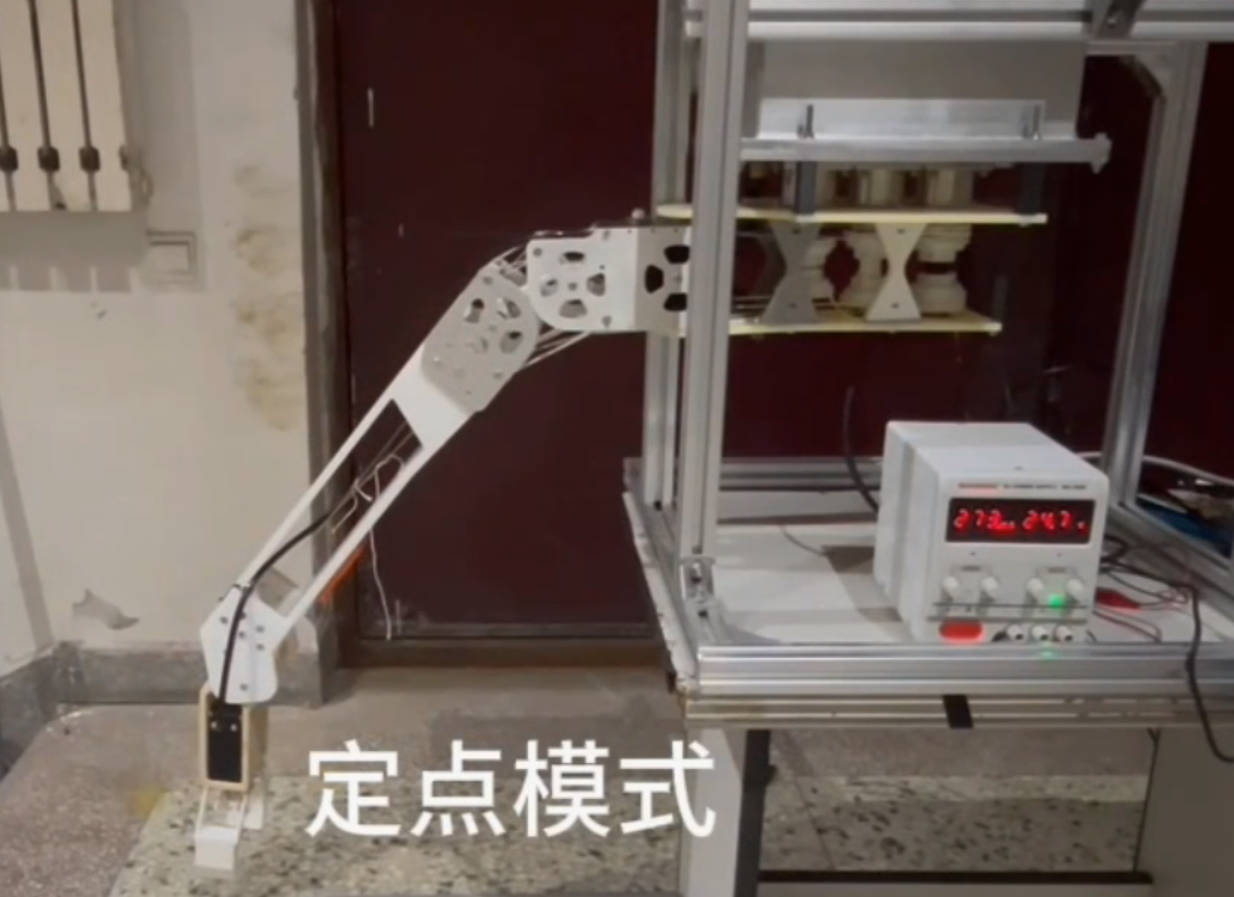
\includegraphics[width = \textwidth]{figures/0.50-0.7.jpg}
        }% 这里写第一张图的英文描述
    \end{minipage}
    % \hfill % 撑开左右间距
    % 第二张子图
    \begin{minipage}{0.45\textwidth}
        \centering
        \subfigure[X:0.5Y:0.0Z:0.6]{\label{fig6:sub2}
            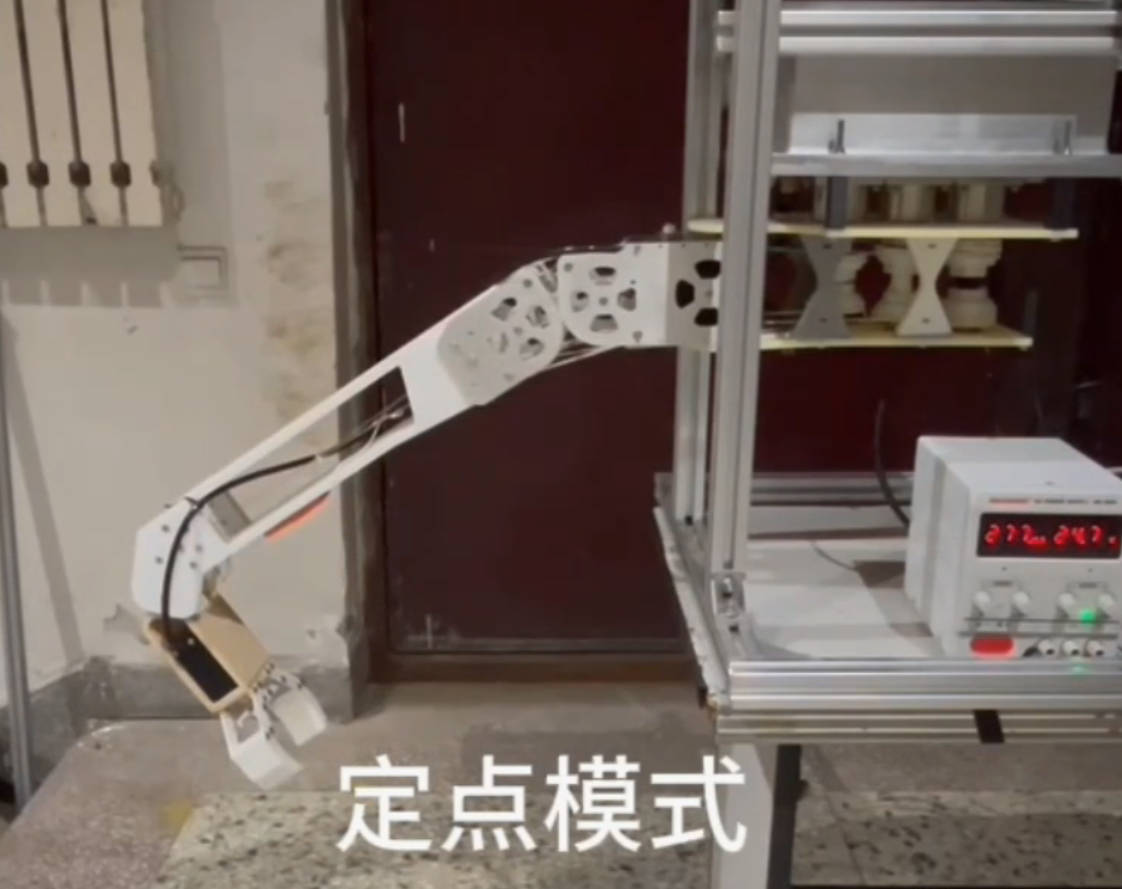
\includegraphics[width = \textwidth]{figures/506.jpg}
        } % 这里写第二张图的英文描述
    \end{minipage}
    \begin{minipage}{0.45\textwidth}
        \centering
        \subfigure[X:0.5Y:0.2Z:0.7]{\label{fig6:sub1}
            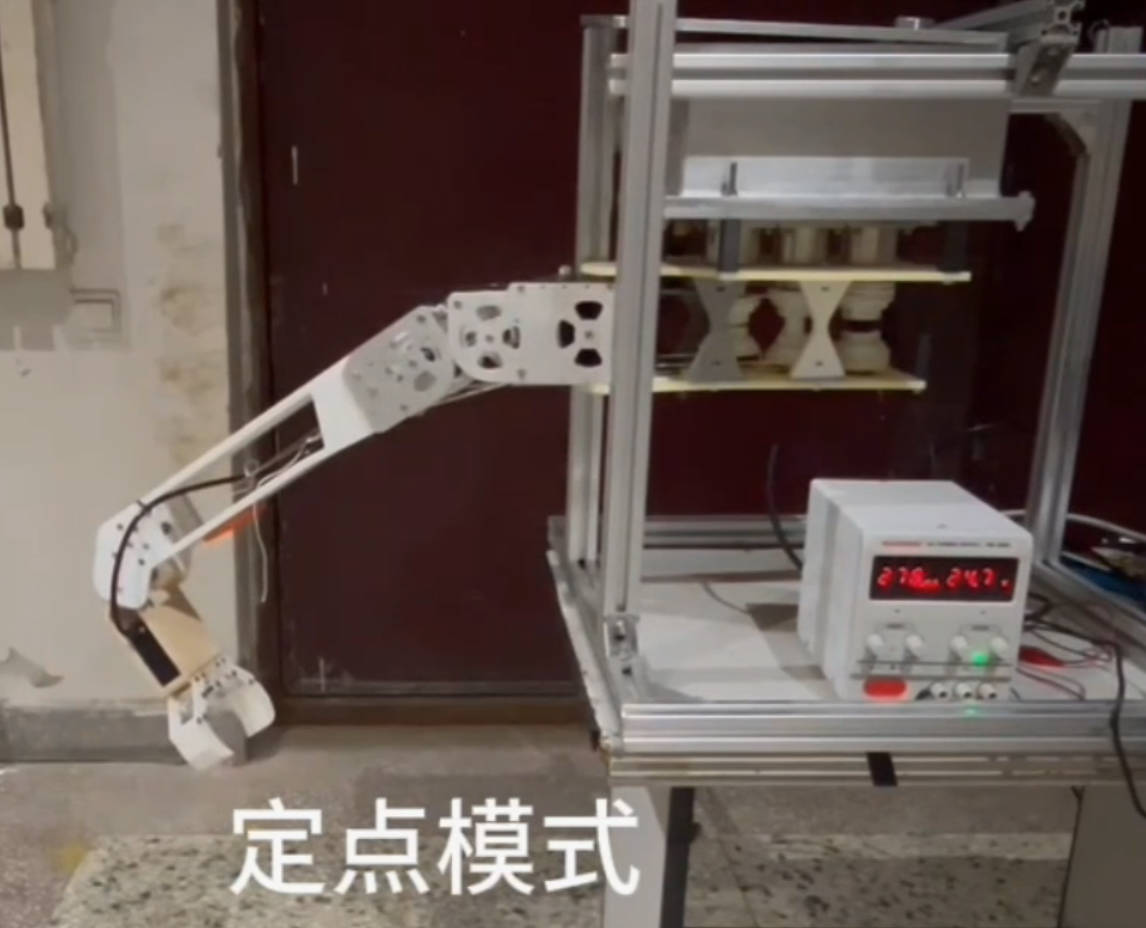
\includegraphics[width = \textwidth]{figures/527.jpg}
        }% 这里写第一张图的英文描述
    \end{minipage}
    % \hfill % 撑开左右间距
    % 第二张子图
    \begin{minipage}{0.45\textwidth}
        \centering
        \subfigure[X:0.5Y:-0.2Z:0.7]{\label{fig6:sub2}
            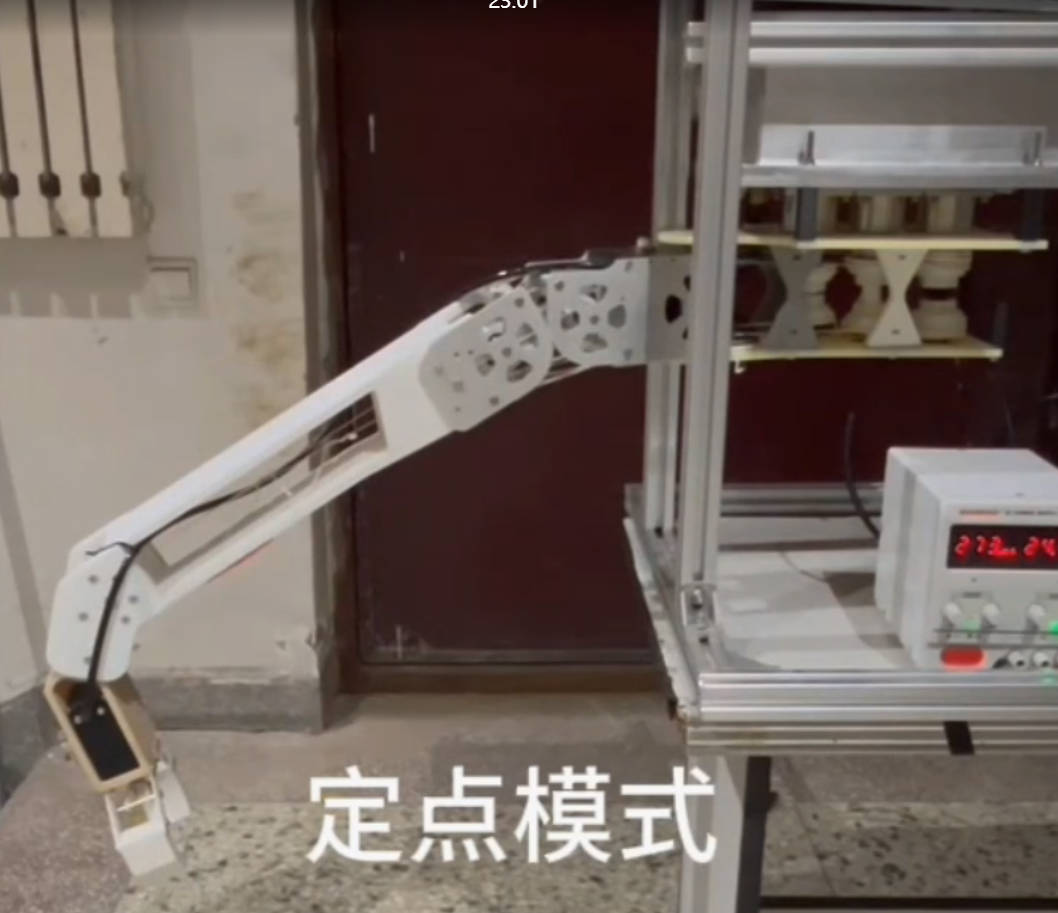
\includegraphics[width = \textwidth]{figures/5227.jpg}
        } % 这里写第二张图的英文描述
    \end{minipage}
    % 中英文总标题
    \caption{基础运动测试}
    \label{fig:total_figure2}
  \end{figure}
然而，通过对实验数据的记录与对比发现，机械臂末端执行器的定位精度存在一定的偏差。分析其原因，主要受以下因素影响：
\begin{itemize}
    \item \textbf{装配与制造公差}：由于机械零件的加工精度及装配过程中的累计误差，导致实际 D-H 参数与理论模型存在偏差。
    \item \textbf{绳索传动特性}：绳驱系统存在的弹性形变与摩擦非线性，在一定程度上影响了末端轨迹的跟随精度。
    \item \textbf{视觉反馈频率}：摄像机分辨率及图像处理链路的延迟对动态抓取过程中的补偿精度产生了一定约束。
\end{itemize}
尽管存在细微精度波动，但整体表现满足设计预期，验证了设计方案的可行性。
\BiSection{本章小结}{Summary}

本章立足于水下绳驱机械臂的样机实验需求，详细阐述了从底层嵌入式硬件到上层分布式软件控制平台的开发过程，并通过实验验证了系统的运动性能与作业可靠性。主要研究内容归纳如下：

\begin{enumerate}
    \item \textbf{软硬件协同控制体系构建}：搭建了以 STM32 微控制器为核心的底层驱动系统，通过设计基于 DMA 循环缓冲与串口空闲中断的通信机制，并引入 CRC-8 数据校验算法，确保了多轴伺服关节控制指令传输的高带宽与高鲁棒性。
    \item \textbf{基于 ROS 2 的分布式软件架构设计}：利用 ROS 2 的模块化解耦合特性，构建了涵盖感知、调度、规划与执行四层逻辑的控制软件平台。实现了基于 ROI 交互的视觉定位模型、标准 G 代码轨迹插补算法以及任务调度状态机，为机械臂的自主作业提供了智能化的软件底座。
    \item \textbf{系统运动性能与视觉抓取验证}：在实验室环境下开展了样机试验。实验结果表明，机械臂能够精准执行复位、空间直线与圆弧轨迹规划等预定任务。视觉引导下的目标抓取实验成功率高，系统反馈链路延迟低，验证了控制方案的有效性。
    \item \textbf{误差来源深度剖析}：通过对比实验数据，分析了装配公差、绳索弹性形变及图像处理延迟对末端定位精度的影响。尽管存在微小偏差，但系统整体运行稳定，满足了设计预期。
\end{enumerate}

本章所构建的软硬件平台不仅验证了水下绳驱机械臂运动学模型及轨迹规划算法的正确性，也为后续开展更复杂环境下（如水下动态环境）的控制策略研究提供了坚实的样机平台与数据支撑。
